\section{Evaluation}

% В данном разделе мы представили результаты апробации трех семантик на нескольких примерах.
In this section, we presented the results of testing three semantics using several examples.

% Для апробации мы реализовали семантики в виде интерпретаторов на языке Хаскелл. В качестве тестировачных программ мы выбрали две простых программы: разворот списка reverso и сортировку списка sorto. А также две более сложных программы: решатель задачи Ханойских башен и решатель задачи Bridge and torch problem.

For evaluation, we implemented semantics in the form of interpreters in the Haskell language. We choose two simple programs as tests: reverse of list and sorting of list. As well as two more complex programs: the Hanoi Towers solver and the Bridge and torch problem solver.

% Для каждой программы мы сделали две версии. Оптимистичная версия --- это программа, в которой мы вручную подобрали оптимальный порядок конъюнктов и пессиместичная версия --- программа с неоптимальным порядком конъюнктов. В последующих диаграммах и таблице указаны средние значения 10 запусков тестов. Также для наивной равномерной конъюнкции мы подобрали количество разверток вручную. Для равномерной конъюнкции, основанной на структурной рекурсии, N было фиксировано и равно 100.
For each program, we made two versions. The optimistic version is a program with optimal conjunct order and the pessimistic version is a program with a non-optimal conjunct order. The following diagrams and table show the average run times of 10 test runs. Also for a naive fair conjunction, we picked up the optimal count of unfolding $N$ manually. For a fair conjunction based on structural recursion, $N$ was fixed at 100.

\begin{figure}
\centering
\begin{minipage}{.5\textwidth}
  \centering
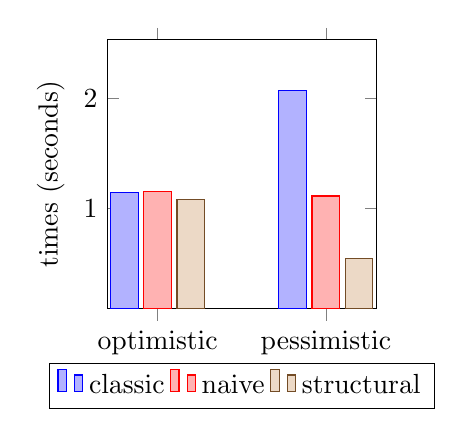
\begin{tikzpicture}
\begin{axis}[
    ybar,
    enlargelimits=0.3,
    width=5cm, height=5cm,
    legend style={at={(0.5,-0.2)},
      anchor=north,legend columns=-1},
    ylabel={times (seconds)},
    symbolic x coords={optimistic, pessimistic},
    xtick=data
    ]
\addplot coordinates {(optimistic,1.142) (pessimistic,2.073)};
\addplot coordinates {(optimistic,1.151) (pessimistic,1.110)};
\addplot coordinates {(optimistic,1.077) (pessimistic,0.542)};
\legend{classic,naive,structural}
\end{axis}
\end{tikzpicture}
  \captionof{figure}{revers$^o$ evaluation for a list with a length of 90}
  \label{fair:plot-reverso}
\end{minipage}%
\begin{minipage}{.5\textwidth}
  \centering
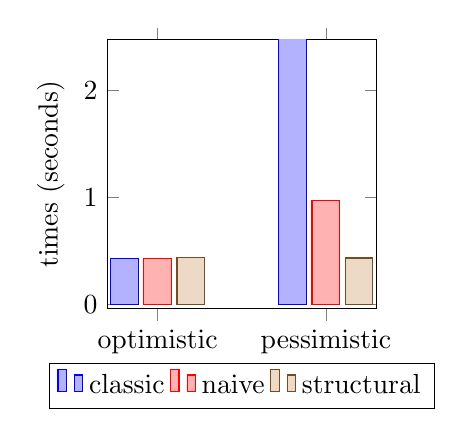
\begin{tikzpicture}
\begin{axis}[
    ybar, ymax = 2,
    enlargelimits=0.3,
    width=5cm, height=5cm,
    legend style={at={(0.5,-0.2)},
      anchor=north,legend columns=-1},
    ylabel={times (seconds)},
    symbolic x coords={optimistic, pessimistic},
    xtick=data
    ]
\addplot coordinates {(optimistic,0.430) (pessimistic,300)};
\addplot coordinates {(optimistic,0.428) (pessimistic,0.969)};
\addplot coordinates {(optimistic,0.433) (pessimistic,0.432)};
\legend{classic,naive,structural}
\end{axis}
\end{tikzpicture}
 \captionof{figure}{sort$^o$ evaluation for a list with a length of 5}
\label{fair:plot-sorto}
\end{minipage}
\end{figure}

\begin{figure}
\centering
\begin{minipage}{.5\textwidth}
  \centering
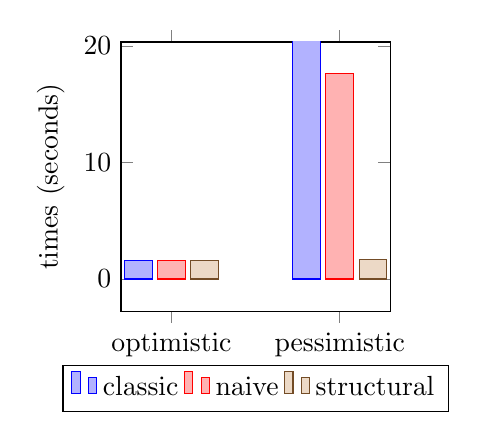
\begin{tikzpicture}
\begin{axis}[
    ybar, ymax = 16,
    enlargelimits=0.3,
    width=5cm, height=5cm,
    legend style={at={(0.5,-0.2)},
      anchor=north,legend columns=-1},
    ylabel={times (seconds)},
    symbolic x coords={optimistic, pessimistic},
    xtick=data
    ]
\addplot coordinates {(optimistic,1.574) (pessimistic,300)};
\addplot coordinates {(optimistic,1.579) (pessimistic,17.604)};
\addplot coordinates {(optimistic,1.585) (pessimistic,1.646)};
\legend{classic,naive,structural}
\end{axis}
\end{tikzpicture}
 \captionof{figure}{``The Tower of Hanoi'' solver evaluation}
\label{fair:plot-hanoi}
\end{minipage}%
\begin{minipage}{.5\textwidth}
  \centering
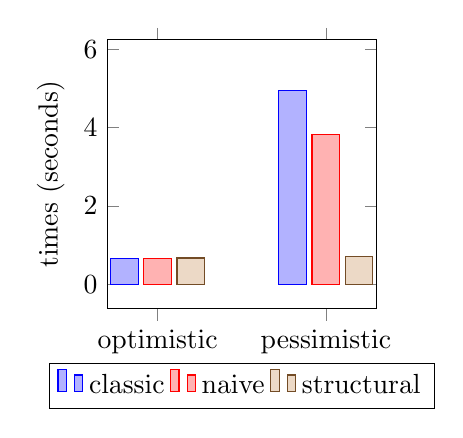
\begin{tikzpicture}
\begin{axis}[
    ybar,
    enlargelimits=0.3,
    width=5cm, height=5cm,
    legend style={at={(0.5,-0.2)},
      anchor=north,legend columns=-1},
    ylabel={times (seconds)},
    symbolic x coords={optimistic, pessimistic},
    xtick=data
    ]
\addplot coordinates {(optimistic,0.669) (pessimistic,4.956)};
\addplot coordinates {(optimistic,0.663) (pessimistic,3.820)};
\addplot coordinates {(optimistic,0.675) (pessimistic,0.712)};
\legend{classic,naive,structural}
\end{axis}
\end{tikzpicture}
 \captionof{figure}{``Bridge and torch problem'' solver evaluation}
\label{fair:plot-bridge}
\end{minipage}
\end{figure}

% На изображениях 12-15 представлены результаты апробации в виде столбцовых диаграмм. В оптимистичном случае результаты схожи для всех семантик. В пессиместичном случае время работы напрпавленной конъюнкции резко возрастает, время работы наивной равномерной конъюнкции также ворзрастает, но не так сильно. Равномерная конъюнкция, основанная на структурной рекурсии, демострирует схожую эффективность в сравнении с оптимистичным случаем.
Figures~\ref{fair:plot-reverso}-\ref{fair:plot-bridge} show the results of approbation in the form of bar charts. In the optimistic case, the results are similar for all semantics. In the pessimistic case, the evaluation time of the directional conjunction rabidly increases, the evaluation time of the naive fair conjunction also increases, but not so much. The fair conjunction based on structural recursion demonstrates similar efficiencies compared to the optimistic case.

% Более подробно результаты представлены на изображении 16. Можно заметить, что время работы программы sorto в пессиместичном случае очень быстро растет с увеличением длины списка для направленной конъюнкции и наивной равномерной. В случае с равномерной конъюнкцией, основанной на структурной рекурсии, пессиместичный случай растет сопостовимо с оптимистичным.
The results are presented in more detail in Figure~\ref{fair:evaluation-table}. It can be noted that the \lstinline{sort$^o$} runtime in the pessimistic case increase very rapidly with increasing list length for directional and naive fair conjunctions. In the case of a fair conjunction based on structural recursion, the pessimistic case increases comparable to the optimistic one.

\begin{figure}[h]
  \small
  \centering
  \begin{tabular}{ c | c | c | c | c | c | c | c }
    \multirow{2}{*}{relation} & \multirow{2}{*}{size} & 
    \multicolumn{2}{c}{directed conjunction} &
    \multicolumn{2}{c}{naive fair conjunction} &
    \multicolumn{2}{c}{structural recursion} \\
    \cline{3-8}
    & & optimistic & pessimistic & optimistic & pessimistic & optimistic & pessimistic  \\ 
    \hline
    \multirow{3}{*}{revers$^o$}
                 & 30   & 0.465 & 0.532 & 0.468 & 0.461  & 0.438 & 0.425 \\
                 & 60   & 0.579 & 0.828 & 0.577 & 0.658  & 0.545 & 0.450 \\
                 & 90   & 1.142 & 2.073 & 1.151 & 1.110  & 1.077 & 0.542 \\
    \hline
    \multirow{5}{*}{sort$^o$}
                 & 3    & 0.418 & 0.432 & 0.420 & 0.420  & 0.424 & 0.425 \\
                 & 4    & 0.424 & 3.924 & 0.424 & 0.455  & 0.429 & 0.429 \\
                 & 5    & 0.430 & >300  & 0.428 & 0.969  & 0.433 & 0.432 \\
                 & 6    & 0.434 & >300  & 0.430 & 11.577 & 0.434 & 0.437 \\
                 & 30   & 1.664 & >300  & 1.636 & >300   & 1.723 & 1.751 \\ 
    \hline
    hanoi$^o$    & -    & 1.574 & >300  & 1.579 & 17.604 & 1.585 & 1.646 \\
    \hline
    bridge$^o$   & -    & 0.669 & 4.956 & 0.663 & 3.820 & 0.675 & 0.712    

  \end{tabular}
  \caption{The results of an evaluation: running times of benchmarks in seconds}
  \label{fair:evaluation-table}
\end{figure}

% Подводя итог, равномерная конъюнкция, основанная на структурной рекурсии сопоставима по эффективности с направленной конъюнкцией. Более того, это конъюнкция слабо зависит от порядка конъюнктов.
To summarize, a fair conjunction based on structural recursion is comparable in performance to a directed conjunction. Moreover, this conjunction weakly depends on the order of the conjuncts.